\typeout{IJCAI--PRICAI--20 Instructions for Authors}
\documentclass{article}
\pdfpagewidth=8.5in
\pdfpageheight=11in
\usepackage{ijcai20}

\usepackage{times}
\usepackage{soul}
\usepackage{url}
\usepackage[hidelinks]{hyperref}
\usepackage[utf8]{inputenc}
\usepackage[small]{caption}
\usepackage{graphicx}
\usepackage{amsmath}
\usepackage{amsthm}
\usepackage{booktabs}
\usepackage{algorithm}
\usepackage{algorithmic}
\urlstyle{same}

\usepackage[table]{xcolor}
\usepackage{graphicx}
\usepackage{amssymb,amsmath,amsthm,amsfonts}
\usepackage[vlined,ruled,linesnumbered,algo2e]{algorithm2e}
\usepackage{color}

\newcommand{\tool}{{\sc BASolver}\xspace}
\newcommand{\ctool}{{\sc MBlocking}\xspace}
\newcommand{\bc}{{\sc BC}\xspace}
\newcommand{\nbc}{{\sc NBC}\xspace}
\newcommand{\bdd}{{\sc BDD}\xspace}



\newtheorem{theorem}{Theorem}
\newtheorem{lemma}{Lemma}
\newtheorem{corollary}{Corollary}
\newtheorem{proposition}{Proposition}
\newtheorem{definition}{Definition}
\newtheorem{example}{Example}
\newtheorem{remark}{Remark}

\begin{document}
\title{Solving ALLSAT with Backbone Information}
\maketitle
\begin{abstract}
The ALLSAT (All-Solutions) problems focus on finding every existing satisfiable assignment of a given propositional formula. Several different tasks in computer science require the finding of all satisfiable assignments, including model checking, automaton translation and test cases generation.
In this paper, we introduce \tool, a backbone based ALLSAT solver for propositional formulas. Comparing to the existing work, \tool uses backbone information to get shorter partial solutions. With more solutions representing in the shorter partial solution, less SAT solving is needed and the efficiency of ALLSAT computing increases.
Experiments show that although finding backbone variables consumes additional computing time , \tool is still faster than existing tools,. including \ctool, \bc, \nbc and \bdd.
Within the time and memory limitation, \tool solves the most formulas.
% (79), \ctool solves 65 formulas, \bc solves 64 formulas, \nbc solves 53 formulas and \bdd solves 51 formulas.
For the formulas that are solved by all the 5 tools, \tool uses the least computing time.
% (9558.64 seconds), which is 51\% less than \ctool(19427.51 seconds), 48\% less than \bc(18221,86 seconds),  54\% less than \nbc(21263.27 seconds) and 67\% less than \bdd(28901.35 seconds). 
\end{abstract}
\section{Introduction}
The SAT (SATisfiable) applications, such as model checking~\cite{bmc,ic3}, program analysis~\cite{klee,cpachecker,cbmc}, network verification ~\cite{lopes2015checking,majumdar2014kuai,zhang2012verification}, quantifier elimination~\cite{brauer2011existential} and predicate abstraction~\cite{lahiri2003symbolic}, have gained considerable attentions due to the increasing capability of modern SAT solvers. 
Also, among several applications like unbounded hardware model checking ~\cite{car}, logic minimization ~\cite{sapra2003sat}, and temporal logic planning ~\cite{aalta}, computing all satisfiable assignments of the model is demanded. This paper focuses on the All-SAT (ALL-SATisfiable) problem, which aims to compute all satisfiable assignment of a propositional formula, and presents an efficient solver \tool to help tackle such problems.

Although the satisfiability of propositional formulas is known as a NP-complete problem, modern SAT solvers are able to find a satisfiable assignment within affordable time. However, directly enumerating all satisfiable assignments of a formula may be infeasible because the number of such assignments can be exponential to the size of the formula. As a result, solving the All-SAT problem remains as a challenging task. As far as we know, there are mainly two kinds of solutions to All-SAT, i.e., the blocking-based~\cite{mcmillan2002applying} and non-blocking-based~\cite{grumberg2004memory}. The blocking-based strategy uses the SAT solver to find a satisfiable assignment, and then blocks such assignment in the original formula so as to avoid finding the same solution repeatedly. Blocking partial assignments instead of the full ones is a common optimization used in the blocking-based solution. The motivation comes from that normally the SAT solver is good at enumerating partial assignments while not at the full ones. 
Meanwhile, the non-blocking solution backtracks the decision diagram inside the SAT solver to find every satisfiable assignment of the given formula. Once a (full) satisfiable assignment is found by the SAT solver, the non-blocking approach backtracks to a previous decision level with some specific strategies and flips the value of the decision variable at that level to generate a new assignment. The All-SAT computation is complete as soon as every branch value of variables in the decision diagram is visited. 
The advantages of the non-blocking strategy are to avoid the changes of the formula and utilizes the full information of the decision diagrams in the SAT solver, while the blocking-based one is more straightforward and the implementation does not require changes to the SAT solver.

\tool follows the blocking-based framework, uses Minisat v2.1.1~\cite{minisat} as the underlying SAT solver and is implemented in C++. The distinguished feature of \tool is to use the backbone information to reduce the sizes of partial assignments and thus the corresponding blocking clauses. It is not hard to prove that removing every backbone variable from the partial assignment and adding it back to the given formula as a unit clause does not affect the satisfying assignment space of the original formula. 
However, the benefit of doing so is, the number of SAT solving in \tool may be reduced as a shorter partial assignment potentially represents a set of more full ones. As a result, the performance of \tool may improve significantly. Although finding backbone variables pays additional cost, \tool performs better than the state-of-the-art tools.

We compared \tool to 4 off-the-shelf solvers, including two blocking-based, i.e., \ctool~\cite{ctool} and \bc, and two non-blocking-based, i.e., \nbc and \bdd~\cite{ietool}. Among all the testing solvers, \tool solves (finds every assignment of the given formula) the largest amount of formulas (79 out of 608) within the given time and memory resources, comparing to the number of 65, 64, 53 and 50 for \ctool, \bc, \nbc and \bdd  respectively. 
For the 30 formulas that can be solved by all the solvers, \tool performs the fastest by saving the percentage of 51\%, 48\%, 54\% and 67\% time cost than \ctool, \bc, \nbc and \bdd respectively.
%For the formulas that are solved by both \tool and \ctool, \tool uses 23\% less computing time than \ctool does.
%\tool uses 37\%, 68\% and 31\% less computing time than \bc, \nbc and \bdd does respectively for the formulas that are mutually solved by \tool and one of the comparing tools.
Finally, \tool uses the minimal blocking clauses among the three blocking-based tools. The average length of blocking clauses in \tool is 1026, which is approximately 5\% of that in \ctool (22182) and 16\% of that in \bc (6180). 

The remainder of the paper is organized as follows. We describe notations and preliminaries in Section \ref{sec:prel}. The algorithms of \tool are discussed in Section \ref{sec:meth}, experimental results are shown in Section \ref{sec:expr} and related work are discussed in Section \ref{sec:rela}. We conclude the paper in Section \ref{sec:conc}.


\section{Preliminaries} \label{sec:prel}
Let $X$ be a finite set of Boolean variables. For every Boolean variable $x\in X$, $x$ can only be assigned to 0 or 1, otherwise the value of $x$ is NOT\_KNOWN.
A literal $l$ is either a Boolean variable $x$ or its negation $\neg x$. For a literal $l$, the corresponding variable of $l$ is $x(l)$.
A clause $c$ is a disjunction of literals, a literal $l$ is in a clause $c$ ($l\in c$) if and only if $l$ appears in the disjunction that compose the clause $c$. A variable $x$ is in a clause $c$ if and only if literal $x$ or literal $\neg x$ is in the clause $c$.
A SAT formula $F$ is a conjunction of clauses, a clause $c$ is in the formula $F$ ($c\in F$) if and only if $c$ appears in the conjunction that compose the formula $F$. A variable $x$ is in a formula $F$ if and only if there exists a clause $c\in F$ such that $x\in c$ or $\neg x\in c$. 

An \emph{assignment} $a$ of a given SAT formula $F$ is a function that maps each variable $x\in F$ to 0, 1, or NOT\_KNOWN. 
For example, an assignment $a: \{x_1, x_2, ..., x_k\} \mapsto \{1, 1, ..., 0\}$ is an assignment of the formula $F$, where $k$ is the number of Boolean variables in $F$. 
For a variable $x\in F$, the value of $x$ in the assignment $a$ is $a(x)$, the value of a clause $c\in F$ in the assignment $a$ is $a(c)$, and the value of $F$ in the assignment $a$ is $a(F)$.
$\neg a(x)=1$ if $a(x)=0$ and $\neg a(x)=0$ if $a(x)=1$.
For an assignment $a$ if there does not exist a variable $x\in F$, such that $a(x)$=NOT\_KNOWN, then $a$ is a full assignment of the given formula $F$. 
An assignment $p$ is a partial assignment if there exists at least one variable $x$ such that $p(x)$=NOT\_KNOWN.

For a given assignment $v$, $v$ is a \emph{solution} of the given formula $F$ if and only if the value of $F$ in the assignment $v$ is 1, i.e., $v\models F$ if and only if $v(F)=1$. If $v$ is a full assignment of $F$ then $v$ is also a full solution of $F$. $v$ is a partial solution of $F$ if $v$ is a partial assignment.
The solutions are written as the conjunctions of literals for short, for example, for a solution $v$ such that $v(a)=1$ and $v(b)=0$, then $v$ is written as $v=a\wedge \neg b$.

For a given partial solution $v$, $v$ is able to represent at least two different full solutions $v_1$ and $v_2$, for every variable $x$ such that $v(x) \neq $NOT\_KNOWN, $v_1(x) = v_2(x) = v(x)$, and for every variable $x'$ such that $v(x')$ = NOT\_KNOWN, $v_1(x') \neq v_2(x')$ and $v_1(x') \neq $ NOT\_KNOWN, $v_2(x') \neq $NOT\_KNOWN.

For example, given a formula $F=(a\vee b)\wedge(a\vee \neg b)$, $v=a$ is partial solution of $F$ and $v_1=a\wedge b$, $v_2=a\wedge \neg b$ are two different full solution represents by $v$.


\begin{definition}[Backbone Variable]
For a given satisfiable formula $F$, and a variable $x\in F$, $x$ is a backbone variable if $x\wedge F$ or $\neg x \wedge F$ is unsatisfiable.
\end{definition}

\begin{lemma}[Backbone Assignment]
For a backbone variable $x$ of a given formula $F$, the value of $x$ must be always assigned to 1 or 0 in all solutions.
\end{lemma}

\begin{definition}[Essential Literals]
For a given formula $F$, a literal $x\in F$ and a full solution $v\models F$, $x$ is an essential literal of $F$ with $v$, if and only if there exists a clause $c\in F$ such that $v(x)=1, x\in c$ and for every other literal $x'\in c, x\neq x'$, $v(x')=0$. 
\end{definition}

An essential variable $x$ is the only reason that make a clause $c$ satisfiable in a formula $F$ with the given solution. For an essential variable $x$ with solution $v$, the assignment $a$ is not a solution of $F$ such that for every variable $x' \neq x $, $a(x')=v(x')$ and $a(x)=\neg v(x)$.

For example, given a formula $F=(a\vee b)\wedge(a \vee \neg b)$, $a$ is a backbone variable since $\neg a \wedge F$ is unsatisfiable.
There are only two solutions of $F$, $v_1=a\wedge b$, and $v_2=a\wedge \neg b$, the assignment of backbone variable $a$ is always 1 in every solution of $F$. 
For the solution $v_1$, the literal $a$ is an essential literal since for the clause $a\vee \neg b$, $v_1(a)=1$ and for every other literal (the literal $\neg b$) in $a\vee \neg b$, $v_1(\neg b)=0$.
\section{All-SAT Solver Using Backbone Techniques} \label{sec:meth}
We propose and implement an All-SAT solver \tool, which uses backbone information to get shorter partial solutions comparing to other tools.
With the help of shorter partial solutions, the number of SAT calls in \tool significantly reduces and the efficiency increases.

\subsection{Overview of Algorithms}
Figure \ref{fig:overflow} shows the workflow of \tool.
Given a formula $F$, \tool first computes the backbone variables of $F$ using tools from \cite{bb}.
For every backbone variable $bl$ of $F$, $bl\in \BL(F)$, and $bl$ is added to $F$ as a unit clause. During the computation of backbone variables, solutions are also generated and stored in $S(F)$. The partial solution of each solution $v\in S(F)$ is stored in $P(F)$.
\tool then computes the partial solution $p=partial(v)$ and the blocking clause $C$ for every solution in $S(F)$, and adds the partial solutions to $P(F)$. 
All backbone variables are removed from the partial solution $p$ of a solution $v$, and every essential but non-backbone literal remains in $p$. If every clause is satisfied with the current $p$, i.e., $\forall c\in F, p(c)=1$, the generation of $p$ completes, otherwise, more literals are added to $p$ based on a greedy strategy.
The blocking clause $C$ of a partial solution $p$ is the negation of $p$. For example, if $p=a\wedge b \wedge c$, then the blocking clause $C$ of $p$ is $C=\neg a \vee \neg b \vee \neg c$.
After generating the blocking clause $C$, $F$ is updated with the conjunction between $F$ and $C$, i.e. $F=F\wedge C$.
If $F\wedge C$ is unsatisfiable, then \tool has found every solution of the formula $F$.
Otherwise, a new solution $v'$ is returned by the SAT solver, \tool then computes the partial solution $p'$ and the blocking clause $C'$ again and updates the formula $F$ with $F\wedge C'$.
The updating of the formula $F$ continues until $F$ is unsatisfiable.
\tool then adds every backbone variable in $\BL(F)$ to every partial solution, and every solution of the given formula $F$ is represented in at least one of the partial solution.


\begin{figure}
    \centering
    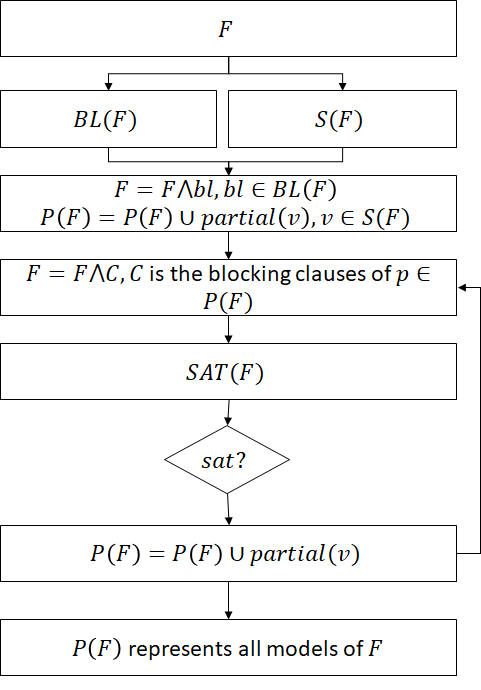
\includegraphics[scale=0.4]{workflow.png}
    \caption{Workflow of \tool}
    \label{fig:overflow}
\end{figure}

\subsection{Algorithms of \tool}
Algorithm \ref{alg:main} shows the main algorithm of \tool, where backbone($F$) uses the algorithms of backbone computing in~\cite{bb}.
The details of blocking($F$) are showed in Algorithm \ref{alg:pc}.
In Algorithm \ref{alg:main}, at Line \ref{ln:P}, the set of partial solutions and blocking clauses are initialized with $\emptyset$. The backbone variables of $F$ is computed, stored in $\BL(F)$ and added to $F$ as unit clauses. The solutions obtained from the backbone computation are stored in $S(F)$.
For every solution $v\in S(F)$, the partial solution $p$ and the blocking clause $C$ are computed and stored in $P(F)$ and $BC(F)$ respectively. 
At Line \ref{ln:bc}, the blocking clauses in $BC(F)$ are added to $F$, $ret$ is assigned with the satisfiability of $F$, returned by the Minisat Solver. If $F$ is satisfiable, then $v$ is a new solution of $F$, the partial solution $p$ and the blocking clause $C$ of the new solution $v$ is computed at Line \ref{ln:cvt}, and $F$ is updated with $F\wedge C$ again. The while loop at Line \ref{ln:check} continues if $F$ is satisfiable, otherwise \tool finishes the computing of every solution for the input formula, which is represented by at least one of the partial solutions in $P(F)$.

\begin{algorithm}
\SetKwInOut{Input}{Input}
\SetKwInOut{Output}{Output}
\SetAlgoShortEnd
\SetFillComment
\Input{A formula $F$}
\Output{Every satisfiable assignments of $F$}
$P(F):=\emptyset$\; \label{ln:P}
$BC(F):=\emptyset$\; \label{ln:BC}
$\BL(F),S(F):=backbone(F)$\; \label{ln:bl}
$F:=F\bigwedge bl, bl\in \BL(F)$\; \label{ln:u}
\ForEach {$v\in S(F)$}{ \label{ln:vt}
	$p,C:=blocking(v)$\; \label{ln:vb}
	$P(F):=P(F)\cup p$\; \label{ln:vp}
	$BC(F):=BC(F)\cup C$\; \label{ln:vbc}
}
$F:=F\bigwedge C, C\in BC(F)$\; \label{ln:bc}
$(ret, v) := SAT(F)$\; \label{ln:check}
\While {ret}{ \label{ln:check-true}
	$p,C:=blocking(v)$\; \label{ln:cvt}
	$P(F):=P(F)\cup p$\; \label{ln:cvb}
	$BC(F):=BC(F)\cup C$\; \label{ln:cvp}
	$F:=F\wedge C$\; \label{ln:cbc}
	$(ret,v):=SAT(F)$\; \label{ln:dc}
}
\Return $P(F)$\; \label{ln:ps}
\caption{Main Algorithm of \tool}\label{alg:main}
\end{algorithm}

In Algorithm \ref{alg:pc}, the partial solutions and the blocking clauses are computed. 
The input of Algorithm \ref{alg:pc} is a formula $F$, the backbone variables $\BL(F)$ of the given formula $F$ and a full solution $v$ returned by the Minisat Solver.
The partial solution $p$ and the blocking clause $C$ of $v$ are initialized as $\emptyset$ at Line \ref{ln:init}.
For every literal $l$ in $v$ such that $v(l)=1$, the algorithm first checks that if $x(l)$ is a backbone variable at Line \ref{ln:check-bl}. If $x(l)$ is a backbone variable, then $l$ is not added to $p$ at this step. Otherwise, $l$ is added to $p$ if there exists a clause $c$ such that $l$ is an essential variable with the given solution $v$ ( $l$ is the only literal in $c$ assigns to $1$ in $v$, from Line \ref{ln:us} to Line \ref{ln:ue}). $\neg l$ is added to the blocking clause $C$ if $l$ is added to the partial solution $p$. 
Starting from Line \ref{ln:cov}, the algorithm checks if every clause $c\in F$ is satisfied by the $p$, i.e., for every clause $c\in F$, there exists at least one literal $l\in c$, and $p(l)=1$. If a clause $c$ is not satisfied by the partial solution $p$, and there does not exist a backbone variable $bl\in c$, $v(bl)=1$, then a literal $l\in c, v(l)=1$ is added to $p$, and the literal $\neg l$ is added to $C$. 
In order to make $p$ a partial solution (instead of a partial assignment) of $v$, all backbone variables are added to $p$ at Line \ref{ln:bl}, but the blocking clauses remain the same since the backbone variables are already added to $F$ as unit clauses.
After executing the loop starting from Line \ref{ln:cov} and the adding of backbone variables at Line \ref{ln:bl}, every clause in $F$ is satisfied by the partial solution $p$, $p$ and $C$ are then returned by Algorithm \ref{alg:pc}.
\begin{algorithm}
\SetKwInOut{Input}{Input}
\SetKwInOut{Output}{Output}
\SetAlgoShortEnd
\SetFillComment
\Input{A formula $F$, a full solution $v\models F$ returned by Minisat Solver, the backbone variables $\BL(F)$ of $F$}
\Output{the partial solution $p$ and the blocking clauses $C$ of $v$}
$p:=\emptyset$\;
$C:=\emptyset$\; \label{ln:init}
\ForEach {$l\in v$}{
	\If {$x(l)\in \BL(F)$}{ continue\;} \label{ln:check-bl}
	\If {$\exists c\in F, l\in c$}{
		unique:=true\; \label{ln:us}
		\ForEach {$l'\neq l, l'\in c$}{
			\If {$v(l')=$}{
				unique:=false\;
				break\;
			}
		}
		\If {unique}{ \label{ln:ue}
			$p:=l\wedge l$\;
			$C:=C\vee \neg l$\;
		}
	}
}
\ForEach {$c\in F, (\not\exists bl\in c, bl\in \BL(F))\wedge(\not\exists l\in p, l\in c)$}{ \label{ln:cov}
	\ForEach {$l'\in c$}{
		$p:=l'\wedge l'$\;
		$C:=C \vee \neg l'$\;
		break\;
	}
}
\ForEach {$bl\in \BL(F)$}{ \label{ln:bl}
	$p:=p\wedge bl$\;
}
\Return $p, C$\;
\caption{Computing the Partial Solutions and the Blocking Clauses}\label{alg:pc}
\end{algorithm}

\begin{theorem} \label{theo:bl}
For a backbone variable $bl$ of a given formula $F$, if a partial solution $p\models F$, then $bl$ is in $p$ and $p(bl)=1$.
\end{theorem}

\begin{proof}
Given a formula $F$ and a backbone variable $bl$ of $F$, suppose there exists a partial solution $p$ such that $p(bl)=$ NOT\_KNOWN. Then there must exist two different solutions of $F$, such that for every variable $x\neq bl$, $v_1(x)=v_2(x)=v(x)$, and $v_1(bl)=\neg v_2(bl)=1$ or $v_1(bl)=\neg v_2(bl)=0$. In both cases, $bl$ is not a backbone variable of $F$ which contradicts with the assumptions that $bl$ is a variable of $F$.
\end{proof}
According to Theorem \ref{theo:bl}, there does not exist a partial solution $p$ such that a backbone variable $bl$ is not in $p$. Therefore, it is correct and essential to add all backbone variables back to every partial solution.
After adding the backbone variables to the original formula, they can be removed from the blocking clauses.

The main contribution of \tool is to use backbone variables in the computing of partial solutions and the blocking clauses. As proved in Theorem \ref{theo:bl}, every backbone variable must appear in every partial solution. Therefore, \tool removes the backbone variables and generates blocking clauses without them in it. To simplify the following SAT solving, backbone variables are used as initial assumptions by adding them back as unit clauses. With shorter blocking clauses, the complexity of the following SAT solving decreases. \tool is more efficient when the number of backbone variables in the formulas are larger. 

With the help of backbone variables, for some of the formulas, All-SAT computing terminates without any blocking clauses.
For a given formula $F$, whenever every clause $c\in F$ is satisfied by at least one backbone literal of $F$, \tool terminates. Since the set of backbones is the only one partial solution that represents every full solution of $F$.

Given a formula $F=(a\vee b)\wedge(a \vee \neg b)\wedge (\neg a \vee c \vee \neg d)$.
Table \ref{tab:comp} shows the All-SAT computing procedure of $F$.
\tool first computes the backbone variables of $F$, $a$ is the backbone variable of $F$, and the solution found during the backbone computing is $v=a\wedge b\wedge c \wedge d$. The partial solution $p$ and the blocking clause $C$ returned by Algorithm \ref{alg:pc} are $p=c$ and $C=\neg c$, respectively. 
Then $F$ is updated with the backbone variables and the blocking clauses, the backbone variable $a$ is added to $F$ as unit clause, and the blocking clause $\neg c$ is also added to $F$. The updated $F$ is $F=(a\vee b)\wedge(a \vee \neg b)\wedge (\neg a \vee c \vee \neg d)\wedge a\wedge \neg c$.
A new solution $v'=a\wedge b\wedge \neg c \wedge \neg d$ for the formula $F$ is computed. $p=\neg d$ and $C=d$ are returned by Algorithm \ref{alg:pc}.
Then $F$ is updated with $F=(a\vee b)\wedge(a \vee \neg b)\wedge (\neg a \vee c \vee \neg d)\wedge a\wedge \neg c\wedge d$. $F$ is unsatisfiable, and the All-SAT computing of $F=(a\vee b)\wedge(a \vee \neg b)\wedge (\neg a \vee c \vee \neg d)$ finished.
The solutions of $F=(a\vee b)\wedge(a \vee \neg b)\wedge (\neg a \vee c \vee \neg d)$ are represented with either $a\wedge \neg c$ or $a\wedge d$.

\begin{table*}
\begin{tabular}{ccccc}
\toprule
Formula & Full Solution & Backbone Variables & Partial Solution & Blocking Clauses \\
\midrule
$(a\vee b)\wedge(a \vee \neg b)\wedge (\neg a \vee c \vee \neg d)$ & $a\wedge b\wedge c\wedge d$ & $a$ & $c$ & $\neg c$ \\
$(a\vee b)\wedge(a \vee \neg b)\wedge (\neg a \vee c \vee \neg d)\wedge a\wedge \neg c$ &  $a\wedge b\wedge c\wedge d$ & $a$ & $\neg d$ & $d$ \\
$(a\vee b)\wedge(a \vee \neg b)\wedge (\neg a \vee c \vee \neg d)\wedge a\wedge \neg c\wedge d$ & Unsatisfiable &  & & \\
\bottomrule
\end{tabular}
    \caption{Computing Procedure of \tool }
    \label{tab:comp}
\end{table*} 



\section{Evaluation} \label{sec:expr}
We implemented \tool based on Minisat v2.1.1, using C++. \tool, \ctool and \bc use the Minisat Solver as an oracle while \nbc and \bdd change the implementation of Minisat according to the algorithms.

The experiments are conducted on clusters with 64GB memory limitation and 10 hours runtime limitation. 
The operating systems are Red-Hat Enterprise Linux. We can not guarantee that the performances of CPUs in the cluster are exactly the same, thus all experiments are repeated 3 times and the average results are computed to enhance fairness. \tool runs sequentially in the experiments and does not use the incremental features in the Minisat Solver.

We use formulas from industrial tracks of SAT competitions from 2011 to 2017 as benchmarks. There are 1816 formulas in total, 552 of them are known as unsatisfiable, 608 of them are satisfiable and the satisfiability of the rest remain unknown. Therefore, the size of the final benchmark is 608. The origin of these formulas includes encryption problems, planning problems, hardware model checking problems and fault localization problems, etc.

\subsection{Overall Performance of the Tools}
Table \ref{tab:main} shows the overall performance of the tools. The first column of Table \ref{tab:main} is the name and the number of the formulas. For clarification, we only include the formulas that at least one of the tools solves them. The second column is the average number of variables, and the third column is the average number of clauses of the formulas. The forth column is the average number of solutions in the formulas. Starting from the fifth column, the number of formulas solve by \tool, \ctool, \bc, \nbc and \bdd are listed respectively.
There are 79 formulas that are solved by at least one of the tools. \tool solves all 79 formulas, \ctool solves 65 formulas, \bc solves 64 formulas, \nbc solves 53 formulas and \bdd solves 51 formulas. For the other 4 comparing tools (\ctool, \bc, \nbc and \bdd), there exists at least one group of formulas that the tools only solve a small part of them. For example, \nbc only solves 1 formula in the Dimacs group, and \ctool failed to solve a formula in the Complete group.
\tool solves the most formulas among the 5 tools, which indicates that the efficiency of \tool is better than the comparing tools with the given benchmark.

\begin{table*}
\begin{tabular}{cccccccccc}
\toprule
Formulas & AveVAR & AveCL & AveFST & \#AveSATInst & \tool & \ctool & \bc & \nbc & \bdd \\
\midrule
Dimacs(15) & 680 & 17079 & 508.14 & 1 & 15 & 15 & 13 & 1 & 15 \\
AProve(2) & 8565 & 28931 & 7.32 & 78 & 2 & 2 & 2 & 2 & 2 \\
Complete(4) & 600 & 27140 & 0.02 & 1 & 4 & 0 & 4 & 4 & 0 \\
Encryption(12) &  8616 & 82773 & 44.75 & 1 & 12 & 10 & 12 & 11 & 6 \\
Manthey(24) & 5179 & 23692 & 780 & 2.58 & 24 & 18 & 14 & 21 & 16 \\
Mp1(12) & 16301 & 185948 & 630.41 & 305.75 & 12 & 11 & 12 & 9 & 8 \\
Others(10) & 11593 & 44557 & 325.19 & 1131 & 10 & 9 & 7 & 5 & 4 \\
Total(79) & 7323 & 393119 & 327.97 & 227.79 & 79 & 65 & 64 & 53 & 51 \\
\bottomrule
\end{tabular}
    \caption{Overall Performance of ALLSAT Computing Tools}
    \label{tab:main}
\end{table*} 

For the 31 formulas that are solved by all the 5 tools, \tool uses the least computing time (9558.64 seconds), which is 51\% less than \ctool (19427.51 seconds), 48\% less than \bc (18221,86 seconds),  54\% less than \nbc (21263.27 seconds) and 67\% less than \bdd (28901.35 seconds).
Since only \tool solves all the 79 formulas, we only compare the computing time among the formulas that are solved by both \tool and one of the comparing tools (including \ctool, \bc, \nbc, and \bdd).

There are 65 formulas solved by both \tool and \ctool, \ctool uses less computing time than \tool for 11 of the formulas, for the rest 54 formulas, \tool uses less computing time. In total, \tool uses 86274.54 seconds and \ctool uses 110932.01 seconds, which is 22\% more than \tool uses.

There are 64 formulas solved by both \tool and \bc, \bc uses less computing time than \tool for 22 of the formulas, for the rest 44 formulas, \tool uses less computing time. In total, \tool uses 92198.9 seconds and \bc uses 110932.01 seconds, which is 37\% more than \tool uses.

There are 53 formulas solved by both \tool and \nbc, \nbc uses less computing time than \tool for 20 of the formulas, for the rest 33 formulas, \tool uses less computing time. In total, \tool uses 28024.15 seconds and \nbc uses 123761.88 seconds, which is 78\% more than \tool uses.

There are 51 formulas solved by \tool of \bdd, \bdd uses less computing time than \tool for 9 of the formulas, for the rest 42 formulas, \tool uses less computing time. In total, \tool uses 74686.244 seconds and \bdd uses 107023.29 seconds, which is 31\% more than \tool uses.

Based on the comparison of number of solved formulas and computing time between \tool and the other comparing tools, we conclude that \tool is able to solve the most formulas with the least computing time, and \ctool ranks the second place in the comparison. 
\bc solved the third most number of formulas.
The \nbc and \bdd tools solve less formulas with more computing time. 
It indicates that for formulas from the industrial benchmark, blocking based tools have advantages than non-blocking based strategies and BDD based strategies.
We then compare the performance of blocking based tools, including \tool, \ctool and \bc.

\subsection{Compassion among Blocking based Tools}

\begin{figure}
    \centering
    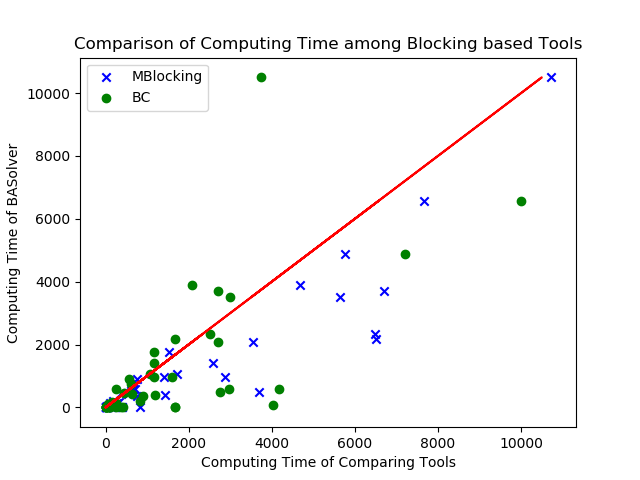
\includegraphics[scale=0.5]{allsat-time.png}
    \caption{Comparison of Computing Time between \tool and Other Tools}
    \label{fig:allsat-time}
\end{figure}

There are 53 formulas that are solved by all the the three tools. Figure \ref{fig:allsat-time} shows the computing time comparison among the 53 formulas. The x-axis is the computing time of the comparing tools, and the y-axis is the computing time of \tool. The line (red) is the base line, set up by the computing time of \tool, the circles (green) are the comparing data of \bc, the crosses (blue) are the computing data of \ctool. For the circles and crosses that are above the line, the computing time of the comparing tools are less than \tool. Results show that for the majority of the formulas, \tool needs less computing time than both \ctool and \bc. And \ctool needs more computing time than \bc on general. It is because that \bc only uses the decision variables in the blocking clauses, therefore, the blocking clauses of \bc is shorter than \ctool. 

Figure \ref{fig:allsat-blk} shows the length of blocking clauses of the three tools. The x-axis is the length of blocking clauses in \ctool and \bc, and the y-axis is the length of blocking clauses in \tool. The line (red) is the base line set up by the length of blocking clauses in \tool, the circles (green) are the comparing data in \bc, and the crosses (blue) are the comparing data in \ctool. The scatter only shows the formulas which average length of blocking clauses is less than 2000. From Figure \ref{fig:allsat-blk}, we can see that for most of the formulas, the length of average blocking clauses in \tool is shorter than \ctool and \bc, which is an important reason that \tool uses less computing time than \ctool and \bc.

With the results of Figure \ref{fig:allsat-time} and \ref{fig:allsat-blk}, we observe that tools with shorter blocking clauses perform better than the ones with longer blocking clauses.
The average length of blocking clauses in \tool is 1026 (among the 79 formulas), the average length of blocking clauses in \ctool is 22182 (among the 65 formulas) and the average length of blocking clauses in \bc is 6180 (among the 64 formulas).
The reason for \tool with short length of blocking clauses is because by using backbone information, a huge part of variables are removed from the blocking clauses. Therefore, backbone information contributes to the computing of ALLSAT problems.

\begin{figure}
    \centering
    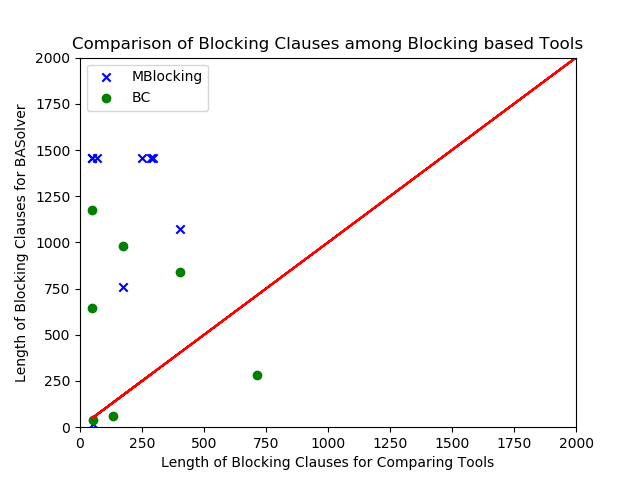
\includegraphics[scale=0.5]{allsat-blk.png}
    \caption{Comparison of Length of Blocking Clauses between \tool and Other Tools}
    \label{fig:allsat-blk}
\end{figure}

%i st bb
% 27.32,34.43,168.48,387.22,953.46,890.8,1406.37,3881.49,5080.45,3508.42,3705.65,6577.17,4876.69,0.02,22.02,9.82,592.7,0.02,592.02,8.81,44.91,59.41,134.19,18.56,112.81,51.46,44.58,18.56,143.73,71.98,51.46,0,0,0.05,2190.72,214.49,494.58,41.27,28.4,421.93,1059.84,2324.63,348.22,967.44,2085.02,5.17,581.39,1777.66,750.19,461.1,12.52,6.33,15.55

% i st blocking
% 50.724706,85.540464,328.695662,1431.727754,2885.069117,746.469704,2585.627846,4692.450813,10711.73746,5651.043807,6709.192745,7665.512216,5760.008729,0.044148,32.382529,11.55542,648.974382,0.143299,697.239595,397.705001,62.550608,130.845185,275.502498,230.81965,262.200193,42.852047,208.340364,25.225832,99.69934,161.046904,172.878436,0.00411,0.010488,0.081907,6499.114935,190.740354,3684.199977,83.985681,133.480907,537.683497,1722.517,6487.315428,764.011712,1406.584865,3547.320029,37.498138,658.131014,1539.000674,604.946888,374.969432,154.215404,385.291636,829.254055

% i st bc
% 75.73,60.59,158.33,1189.73,1171.08,560.48,1165.73,2081.53,3738.13,2989.81,2709.9,10005.95,7206.26,0.01,104.28,57.2,245.39,0.04,2981.58,360.28,48.64,75.24,158.93,18.02,63.37,241.44,59.02,247.22,261.27,4026.74,27.7,0,0,0.08,1680.67,839.03,2756.77,41.02,1665.14,630.75,1062.46,2524.73,913.3,1595.89,2706.84,55.84,4174.49,1177.78,615.5,440.08,107.67,418.03,1665.82

% blk bb
% 54,3069,714,403,132,69184.8,48,248.619256,284.5,66.85714286,48,294.4743802,173.25

% blk bc
% 41,2061,285,841,62,2210,643,31933,299335,15284,1173,56597,979

% blk blocking
% 19,8567,8564,1075,3842,11520,1458,1458,1458,1458,1458,1458,760




\section{Related Work} \label{sec:rela}
There are mainly two kinds of All-SAT solvers, blocking based solvers and non-blocking based solvers.
\tool is a blocking based All-SAT solver.
The main difference between blocking based and non-blocking based solvers is the use of blocking clauses.
In order to avoid finding the already known solutions of the formula, blocking based tools generate the blocking clauses of each known solution and added the blocking clauses back to the solver.
In the non-blocking based All-SAT computing tools \cite{zhao2009asig} \cite{grumberg2004memory} \cite{jabbour2014extending} \cite{ietool}, backtrack techniques in the search tree are used to find more solutions of the given formula. Once a solution is found, the non-blocking based tools choose a decision level and backtracks the search tree to that level. A Different decision is made at that level and a new search path is generated based on the new decision.

A naive blocking based tool \cite{mcmillan2002applying} uses a SAT solver to find a solution of the given formula, then added the negation of the found formula as a blocking clause to the solver.

\ctool\cite{ietool} is another blocking based tool that uses the greedy strategy named minimal blocking strategy to generate the blocking clauses.
For a solution of the given formula, \ctool either computes the set of dominate variables based on the clauses coverage or the set of decision variables and their corresponding reason variables based on the search tree.
Comparing to \ctool, \tool uses backbone information instead of decision variables to generate the blocking clauses. By using backbone variables, shorter blocking clauses are generated.

\nbc\cite{ietool} is a non-blocking based tool that backtracks the search tree to find every solution of the given formula. There are 4 different backtrack strategies in \nbc, and by use these strategies in different orders, there are 8 different strategies in total in \nbc. Each strategy performs differently on the formulas, therefore, the choice of strategies is a challenge for \nbc. 
Comparing to \nbc, \tool only uses one strategy which is backbone variables to find every solution of the formula.

Another two approaches of All-SAT computing are BDD based tools and P systems based tools. The idea of the \bdd is to build an ordered binary decision tree, based on the OBDD, every solution is visited. But the building of the OBDD may take longer computing time than the pure computing of All-SAT and the fixed order of the OBDD also affects the performance of \bdd.
P system based tools use P system to compute NP problems, including All-SAT problems. P system are inherently paralleled and has been used in the solving of SAT problems recently~\cite{p}. Ping~\cite{pa} designs a family of P system and reduce the time complexity of All-SAT computing to linear time. There are only theoretical algorithms and no experiment is conducted in the paper.

\section{Conclusion} \label{sec:conc}
We proposed an All-SAT computing tool \tool which uses backbone information to get shorter blocking clauses and achieve higher efficiency.
Comparing to other All-SAT computing tools, \tool removes backbone variables from the blocking clauses. With shorter blocking clauses, the complexity of the following SAT solving decreases, the number of SAT solving needed decreases and the efficiency of All-SAT computing improves. 
Experiments show that within the given computing time and memory limitation, \tool is able to solver more formulas than other comparing tools.
For the formulas that are solved both by \tool and the comparing tools, \tool uses less computing time than the comparing tools.
Therefore, \tool is an efficient All-SAT computing tool that performs the best among the existing tools with the given benchmark.

\bibliographystyle{named}
\bibliography{ijcai20}

\end{document}
